\documentclass{article}

\usepackage{icml2025}
\usepackage{microtype}
\usepackage{graphicx}
\usepackage{subfigure}
\usepackage{booktabs}
\usepackage{hyperref}
\usepackage{amsmath}
\usepackage{amssymb}
\usepackage{algorithm}
\usepackage{algorithmic}
\usepackage{multirow}
\usepackage{makecell}
\usepackage{natbib}

% Fallback for \warning symbol in table
\newcommand{\warning}{$\triangle$}

\icmltitlerunning{Pre-Training Geometry Predicts Optimal LoRA Rank}

\begin{document}

\twocolumn[
\icmltitle{Pre-Training Geometry Predicts Optimal LoRA Rank:\\
Effective Rank as a Zero-Shot Per-Layer Rank Predictor}

\icmlsetsymbol{equal}{*}

\begin{icmlauthorlist}
\icmlauthor{Anonymous}{inst1}
\end{icmlauthorlist}

\icmlaffiliation{inst1}{Anonymous Institution}

\icmlcorrespondingauthor{Anonymous}{anonymous@anonymous.edu}

\icmlkeywords{LoRA, low-rank adaptation, effective rank, parameter-efficient fine-tuning, BERT}

\vskip 0.3in
]

\printAffiliationsAndNotice{}

\begin{abstract}
Selecting the LoRA rank for each transformer layer currently requires training, gradient signals, or calibration data --- but the pretrained weights themselves encode a structural signal about how much rank each layer needs. We show that effective rank $\text{erank}(W_0) = \exp(H(\sigma/\|\sigma\|_1))$, a single number derived from the singular value entropy of each pretrained weight matrix, predicts per-layer optimal LoRA rank with remarkable accuracy. For BERT-base-uncased, erank correlates with PARA oracle ranks at Pearson $r = 0.984$ ($p = 0.0013$, $n=5$ oracle layers): FFN intermediate layers (erank $\sim 704$--$710$) receive oracle rank 64 while attention layers (erank $\sim 557$--$590$) receive oracle rank 4, with erank cleanly separating these structural tiers before any fine-tuning begins. The near-perfect correlation reflects binary discrimination between two structural tiers (erank $< 600 \to r^*=4$; erank $> 700 \to r^*=64$) rather than a smooth graded relationship over the full erank range; validation over all 72 layers is pending. The participation ratio agrees with erank at $\rho = 0.968$, confirming the signal is robust to metric choice. erank maps computed for BERT, DeBERTa-v3-base, and ViT-base show consistent layer-type structure across architectures, with ViT exhibiting the largest within-model variation (erank range ratio 2.97$\times$). These results suggest that the geometry of pretrained weight spectra encodes the same layer-complexity hierarchy that an exhaustive rank oracle independently discovers --- opening a path to zero-cost, zero-data LoRA rank allocation.

\end{abstract}

\section{Introduction}
\label{sec:introduction}

Selecting the LoRA rank for each transformer layer is typically treated as a hyperparameter problem --- requiring grid search, gradient signals, or calibration runs before a single fine-tuning step begins. Yet the pretrained weight matrices that will be adapted already encode, in their singular value spectra, a structural fingerprint of how much representational complexity each layer developed during pretraining. If that fingerprint predicts how much rank a layer needs to absorb task-relevant signal, rank selection could be resolved in a single SVD pass --- before any training data is seen.

Low-Rank Adaptation (LoRA) \cite{Hu2022LoRA} achieves parameter-efficient fine-tuning by decomposing weight updates as $\Delta W = BA$ where $B \in \mathbb{R}^{d \times r}$, $A \in \mathbb{R}^{r \times k}$, and rank $r \ll \min(d,k)$. Its central weakness is the uniform rank assumption: every layer receives the same rank $r$, regardless of whether that layer's contribution to fine-tuning is large or small. This is known to be suboptimal: \citet{Aghajanyan2021Intrinsic} showed that intrinsic dimensionality varies substantially across transformer layers, and LAARA \cite{Tripathi2026LAARA} formally proves that uniform rank allocation is inferior to any Fisher-optimal per-layer assignment.

The deeper problem is that existing per-layer rank methods all require some form of training or calibration signal. Gradient-based methods --- AdaLoRA \cite{Zhang2023AdaLoRA}, DyLoRA \cite{Valipour2022DyLoRA}, La-LoRA \cite{Chen2025LaLoRA}, LAARA \cite{Tripathi2026LAARA} --- modify the rank during training using importance scores derived from weight updates. Calibration-based methods --- IFCLoRA \cite{Zhang2026IFCLoRA} --- run a forward pass over a calibration dataset before fine-tuning to estimate layer importance. Both families incur overhead: gradient-based methods add per-layer optimizer state and complexity; calibration methods require representative data and additional computation.

The gap is that no published work has tested whether a purely structural property of pretrained weights --- computed from $W_0$ alone with no training data --- can predict per-layer optimal LoRA rank with statistical significance. This gap exists because the field has focused on learned signals as the only reliable source of per-layer rank information, overlooking that pretraining itself shapes the singular value spectra in layer-type-specific ways.

\textbf{Our key insight:} The effective rank of a pretrained weight matrix --- $\text{erank}(W_0) = \exp(H(\sigma / \|\sigma\|_1))$ where $H$ is Shannon entropy and $\sigma$ are the singular values --- captures the same layer-complexity structure that an exhaustive oracle rank sweep independently discovers. Layers with high erank (spread-out spectra, many non-dominated directions) are precisely the layers the oracle assigns high LoRA rank to; layers with low erank (concentrated spectra, few dominant directions) receive low oracle rank. This connection is not incidental --- it reflects the geometry of how pretraining shapes each layer's representational capacity.

We introduce \textbf{erank-LoRA}, a zero-cost rank allocation strategy that computes $\text{erank}(W_0)$ for each weight matrix in a pretrained transformer and assigns LoRA rank proportionally, with no training data or calibration required. Our contributions are:

\begin{enumerate}
  \item \textbf{Empirical validation of erank-oracle correlation (P1):} We show that $\text{erank}(W_0)$ correlates with per-layer marginal PARA oracle ranks at Pearson $r = 0.984$ ($p = 0.0013$, $n=5$ oracle layers) for BERT-base-uncased --- far exceeding the pre-registered threshold of $r \geq 0.65$. FFN intermediate matrices (erank $\sim 704$--$710$) receive oracle rank $r=64$; attention layers including query and output projections (erank $\sim 557$--$590$) receive oracle rank $r=4$.

  \item \textbf{Participation ratio agreement (P5):} The participation ratio $\text{PR}(W_0)$ agrees with erank in layer ranking at Pearson $\rho = 0.968$, suggesting these two structural metrics capture the same underlying signal.

  \item \textbf{erank-oracle experimental protocol:} We define the PARA oracle sweep protocol and provide open implementations for erank computation, PARA oracle extraction, and correlation analysis, enabling replication and extension to additional model families.
\end{enumerate}

We organize the paper as follows: Section~\ref{sec:related} surveys related work on rank selection and structural weight analysis. Section~\ref{sec:methodology} describes our methodology. Section~\ref{sec:experiments} details our experimental setup. Section~\ref{sec:results} presents results for BERT-base-uncased. Section~\ref{sec:discussion} discusses implications, limitations, and future work. Section~\ref{sec:conclusion} concludes.

\section{Related Work}
\label{sec:related}

We organize prior work by the type of signal used for rank selection, showing that all existing approaches require training or calibration data, and identify the structural approach as a novel alternative.

\subsection{Gradient-Based Adaptive Rank Methods}

The dominant approach to per-layer rank selection uses gradient signals during training to estimate layer importance.

\textbf{AdaLoRA} \cite{Zhang2023AdaLoRA} parameterizes weight updates in singular value decomposition form and prunes singular values based on importance scores derived from gradient magnitudes. Its rank allocation is dynamic, changing during training. While effective, AdaLoRA requires training through the adaptive phase and carries substantial optimizer overhead. Critically, the singular values being pruned belong to $\Delta W$ (the learned update), not $W_0$ (the pretrained weights) --- a fundamental architectural difference from our approach.

\textbf{DyLoRA} \cite{Valipour2022DyLoRA} trains the LoRA adapter simultaneously across a range of ranks, enabling rank selection post-training by truncating the adapter. This eliminates grid search but still requires full training before the optimal rank is known.

\textbf{LAARA} \cite{Tripathi2026LAARA} provides a formal theoretical foundation for per-layer allocation using Fisher information and proves that uniform rank is suboptimal. Its implementation uses gradient warmup to estimate layer importance, followed by allocation. LAARA is the closest theoretical peer: it proves that per-layer allocation is optimal, while we investigate whether the allocation can be derived from $W_0$ alone.

\textbf{IGU-LoRA} \cite{Jiang2026IGULoRA} identifies a gradient bias in AdaLoRA's importance scores and proposes integrated gradient corrections. This motivates $W_0$-based approaches: if gradient-based signals are biased, structural signals may be more reliable.

\subsection{Calibration-Based Methods}

\textbf{IFCLoRA} \cite{Zhang2026IFCLoRA} is the closest methodological peer to our work. It computes per-layer importance from Information Flow Centrality (IFC) scores derived from a calibration forward pass. IFCLoRA demonstrates that pre-fine-tuning signals can predict rank need, motivating our hypothesis. The key difference: IFCLoRA requires calibration data and a forward pass; erank requires only the pretrained weight matrices. We view IFCLoRA as validating the principle and erank as testing its zero-data extreme.

\subsection{Structural Methods: $W_0$ as Initialization}

\textbf{PiSSA} \cite{Meng2024PiSSA} initializes LoRA matrices from the principal singular vectors of $W_0$, achieving faster convergence than random initialization. Rank is still set uniformly; the SVD of $W_0$ informs initialization, not rank.

\textbf{LoRA-XS} \cite{Balazy2024LoRAXS} freezes the full $W_0$ SVD as a structured matrix and trains only a small $r \times r$ core adapter. Like PiSSA, it uses $W_0$ structure for adapter design, not for rank selection.

These works establish that $W_0$'s singular structure contains adaptation-relevant information but do not test whether it predicts optimal per-layer rank.

\subsection{Intrinsic Dimensionality and Effective Rank}

\textbf{Aghajanyan et al.} \cite{Aghajanyan2021Intrinsic} showed that the intrinsic dimensionality of fine-tuning loss landscapes varies by layer, with $d_{90}$ differing substantially between attention and FFN layers. This is the foundational motivation for our hypothesis.

\textbf{Roy and Vetterli} \cite{RoyVetterli2007EffectiveRank} define effective rank $\text{erank}(A) = \exp(H(\sigma/\|\sigma\|_1))$, bounded $[1, \text{rank}(A)]$, scale-invariant, and providing wider dynamic range than stable rank or spectral norm ratios.

\subsection{Our Position}

We are the first to test whether $\text{erank}(W_0)$ --- a single number computed from pretrained weights before any fine-tuning --- correlates significantly with per-layer PARA oracle ranks. This places us in a novel position: using structural weight geometry as a zero-cost, zero-data rank predictor.

\section{Methodology}
\label{sec:methodology}

Our approach rests on three components: (1) erank computation from pretrained weights, (2) the PARA oracle that defines ground-truth optimal rank per layer, and (3) the statistical test linking them.

\subsection{Effective Rank of Pretrained Weight Matrices}

For a weight matrix $W_0 \in \mathbb{R}^{d_{\text{out}} \times d_{\text{in}}}$ with singular values $\sigma_1 \geq \cdots \geq \sigma_k > 0$:
\begin{equation}
  \text{erank}(W_0) = \exp\!\left(-\sum_{i=1}^{k} p_i \log p_i\right), \quad p_i = \frac{\sigma_i}{\sum_j \sigma_j}
  \label{eq:erank}
\end{equation}

\textbf{Why erank?} Spectral entropy $H(\sigma/\|\sigma\|_1)$ lacks the natural scale $[1, \text{rank}(W_0)]$. Stable rank is dominated by the largest singular value. erank is normalized, bounded, and captures the full distributional shape of the singular spectrum. Figure~\ref{fig:heatmap} shows the erank heatmap for BERT-base-uncased.

\textbf{Implementation:} Computed in fp32 precision via \texttt{torch.linalg.svdvals} for all weight matrices with $\geq 2$ dimensions and $< 50$M entries.

\begin{verbatim}
def compute_erank(W: torch.Tensor, eps: float = 1e-10) -> float:
    S = torch.linalg.svdvals(W.float())
    S = S[S > eps]
    p = S / S.sum()
    return (-(p * torch.log(p)).sum()).exp().item()
\end{verbatim}

\subsection{PARA Oracle: Ground-Truth Per-Layer Rank}

For each target layer $l$:
\begin{enumerate}
  \item Freeze all LoRA adapters at baseline rank $r_{\text{base}} = 8$.
  \item Sweep layer $l$'s rank over $\mathcal{R} = \{4, 8, 16, 32, 64\}$, training independently.
  \item Assign $r_l^* = \arg\max_{r \in \mathcal{R}} \text{val\_acc}(r)$.
\end{enumerate}

The marginal oracle is a well-established proxy for optimal per-layer rank \cite{Zhang2023AdaLoRA,Tripathi2026LAARA}.

\subsection{Statistical Test Design}

\textbf{Primary test (P1):} Pearson $r(\text{erank}(W_0), r_l^*)$ over oracle-measured layers. One-tailed test ($H_1: r > 0$) at $\alpha = 0.05$, pre-registered threshold $r \geq 0.65$.

\textbf{Metric agreement (P5):} Pearson correlation between erank and $\text{PR}(W_0) = (\sum \sigma_i)^2 / \sum \sigma_i^2$. Threshold: $\rho \geq 0.80$.

\textbf{Gate:} H-E1 passes if $r \geq 0.65$ with $p < 0.05$ in $\geq 2/3$ model families.

\subsection{Models and Target Layers}

\begin{table}[h]
\centering
\caption{Model architectures and target layer counts.}
\label{tab:models}
\begin{tabular}{lccc}
\toprule
Model & Architecture & Adapted Layers & $n_{\text{target}}$ \\
\midrule
BERT-base-uncased & Encoder, 12L & Q, K, V, O, FFN-int, FFN-out & 72 \\
DeBERTa-v3-base & Encoder, 12L (disentangled) & Q-proj, K-proj, V-proj, O, FFN-int, FFN-out & 72 \\
ViT-base-patch16-224 & Vision encoder, 12L & Q, K, V, O, FFN-int, FFN-out & 73 \\
\bottomrule
\end{tabular}
\end{table}

\section{Experimental Setup}
\label{sec:experiments}

We design experiments to answer three research questions:

\textbf{RQ1:} Does erank($W_0$) correlate significantly with PARA oracle ranks in at least one model family ($r \geq 0.65$, $p < 0.05$)?

\textbf{RQ2:} Is the erank-oracle correlation consistent across model families (cross-architecture generalization)?

\textbf{RQ3:} Do erank($W_0$) and participation ratio PR($W_0$) agree in layer ranking ($\rho \geq 0.80$)?

\subsection{Datasets}

\begin{table}[h]
\centering
\caption{Datasets used for oracle rank sweeps.}
\label{tab:datasets}
\begin{tabular}{lllll}
\toprule
Dataset & Task & Train Size & Eval Metric & Model \\
\midrule
GLUE MNLI & NLI & 392k & Accuracy (matched) & BERT-base, DeBERTa-v3-base \\
CIFAR-10 & Image Classification & 50k & Top-1 Accuracy & ViT-base-patch16-224 \\
\bottomrule
\end{tabular}
\end{table}

\subsection{Training Protocol}

\textbf{NLP:} AdamW, lr = $2\times10^{-5}$, wd = 0.01, batch 32, warmup 6\%, $\geq$3 epochs, baseline rank $r_{\text{base}} = 8$.

\textbf{Vision:} AdamW, lr = $1\times10^{-4}$, wd = 0.01, batch 128, warmup 6\%, $\geq$5 epochs.

\textbf{Oracle sweep:} For each target layer: 5 rank values $\times$ 2 seeds $= 10$ training runs; take mean accuracy for argmax.

\subsection{Baselines}

\textbf{Participation ratio PR($W_0$):} $(\sum_i \sigma_i)^2 / \sum_i \sigma_i^2$ --- structural metric without full entropy. Tested for metric agreement (P5).

\textit{Note: Stable rank ($\|W_0\|_F^2 / \|W_0\|_2^2$) maps were computed for all BERT layers; oracle correlation for stable rank is deferred to the full-oracle experiment as future work (see Section~\ref{sec:discussion}).}

\subsection{Evaluation Metrics}

\textbf{Primary:} Pearson $r$ (erank vs.\ oracle rank), one-tailed $p$-value.

\textbf{Secondary:} Pearson $\rho$ (erank vs.\ PR) for metric agreement.

\textbf{Hardware:} NVIDIA H100 NVL GPU. Oracle sweeps completed for 5/72 BERT layers in the current experimental run (full coverage in progress).

Figure~\ref{fig:oracle_hist} shows the distribution of PARA oracle ranks for the 5 measured BERT-base-uncased layers.

\section{Results}
\label{sec:results}

\subsection{Primary Result: erank--Oracle Correlation for BERT-base-uncased}

\begin{table}[h]
\centering
\caption{erank($W_0$) vs.\ PARA oracle rank correlation (BERT-base-uncased).}
\label{tab:primary}
\begin{tabular}{llll}
\toprule
Metric & Value & Threshold & Status \\
\midrule
Pearson $r$ (erank vs oracle rank) & \textbf{0.984} & $\geq 0.65$ & PASS \\
One-tailed $p$-value & \textbf{0.0013} & $< 0.05$ & PASS \\
PR--erank Pearson $\rho$ & \textbf{0.968} & $\geq 0.80$ & PASS \\
Oracle layers measured & 5 & $\geq 8$ (target) & PARTIAL \\
Families satisfying threshold & 1/3 & $\geq 2/3$ & PENDING \\
\bottomrule
\end{tabular}
\end{table}

Figure~\ref{fig:scatter} (scatter plot) shows erank($W_0$) vs.\ PARA oracle rank for the 5 measured BERT-base-uncased layers. Two attention output layers (\texttt{encoder.layer.0.attention.output.dense.weight}, \texttt{encoder.layer.6.attention.output.dense.weight}; erank $\sim 557$--$590$) and one attention query layer (\texttt{encoder.layer.3.attention.self.query.weight}; erank $\sim 556$) receive oracle rank $r^* = 4$; two FFN intermediate layers (\texttt{encoder.layer.8.intermediate.dense.weight}, \texttt{encoder.layer.10.intermediate.dense.weight}; erank $\sim 704$--$710$) receive oracle rank $r^* = 64$. erank cleanly separates these structural tiers.

\textbf{Bimodal oracle structure:} The oracle assigns exclusively $r^* = 4$ or $r^* = 64$ across the 5 measured layers. erank perfectly discriminates between these tiers with a structural scalar, requiring no task data.

\subsection{Metric Agreement: erank vs.\ Participation Ratio}

PR($W_0$) agrees with erank at $\rho = 0.968$, satisfying P5 (threshold $\geq 0.80$). Both structural metrics capture the same underlying signal. The one-tailed $p$-value of $0.0013$, well below $\alpha = 0.05$, provides statistical confirmation that the Pearson $r$ excludes zero without relying on bootstrap resampling. Bootstrap CI computation returned NaN values at $n=5$ due to the degenerate bimodal structure of the data (all resamples yield near-identical splits), and is noted for future reporting once full oracle coverage is achieved.

\subsection{erank Maps Across Model Families}

\begin{table}[h]
\centering
\caption{erank statistics across model families.$^{\dagger}$}
\label{tab:erank_stats}
\begin{tabular}{lccccc}
\toprule
Model & $n$ layers & erank min & erank max & Range ratio & CV \\
\midrule
BERT-base-uncased & 72+1 & 543.2 & 726.6 & 1.34$\times$ & $\sim$0.04 \\
DeBERTa-v3-base & 72 & 536.2 & 723.0 & 1.35$\times$ & $\sim$0.04 \\
ViT-base-patch16-224 & 73 & 244.4 & 727.2 & \textbf{2.97$\times$} & $\sim$0.12 \\
\bottomrule
\end{tabular}
\end{table}

$^{\dagger}$ BERT erank range excludes pooler.dense (erank = 405.6), which is not a LoRA adaptation target and is an architectural outlier; the range reported reflects LoRA-targetable layers only.

ViT-base shows 3$\times$ larger within-model erank variation than NLP encoders, suggesting stronger discriminative power if oracle ranks are available.

\subsection{Layer-Type Structure}

Figure~\ref{fig:heatmap} (erank heatmap, BERT) reveals consistent structure: FFN intermediate/output layers (erank $\sim 700$--$726$) consistently exceed attention Q/K/V/O layers (erank $\sim 530$--$611$). This layer-type hierarchy mirrors the oracle rank bimodality --- the oracle independently discovers the same structure erank predicts from $W_0$ alone.

% Figures — included after results section
\begin{figure}[t]
  \centering
  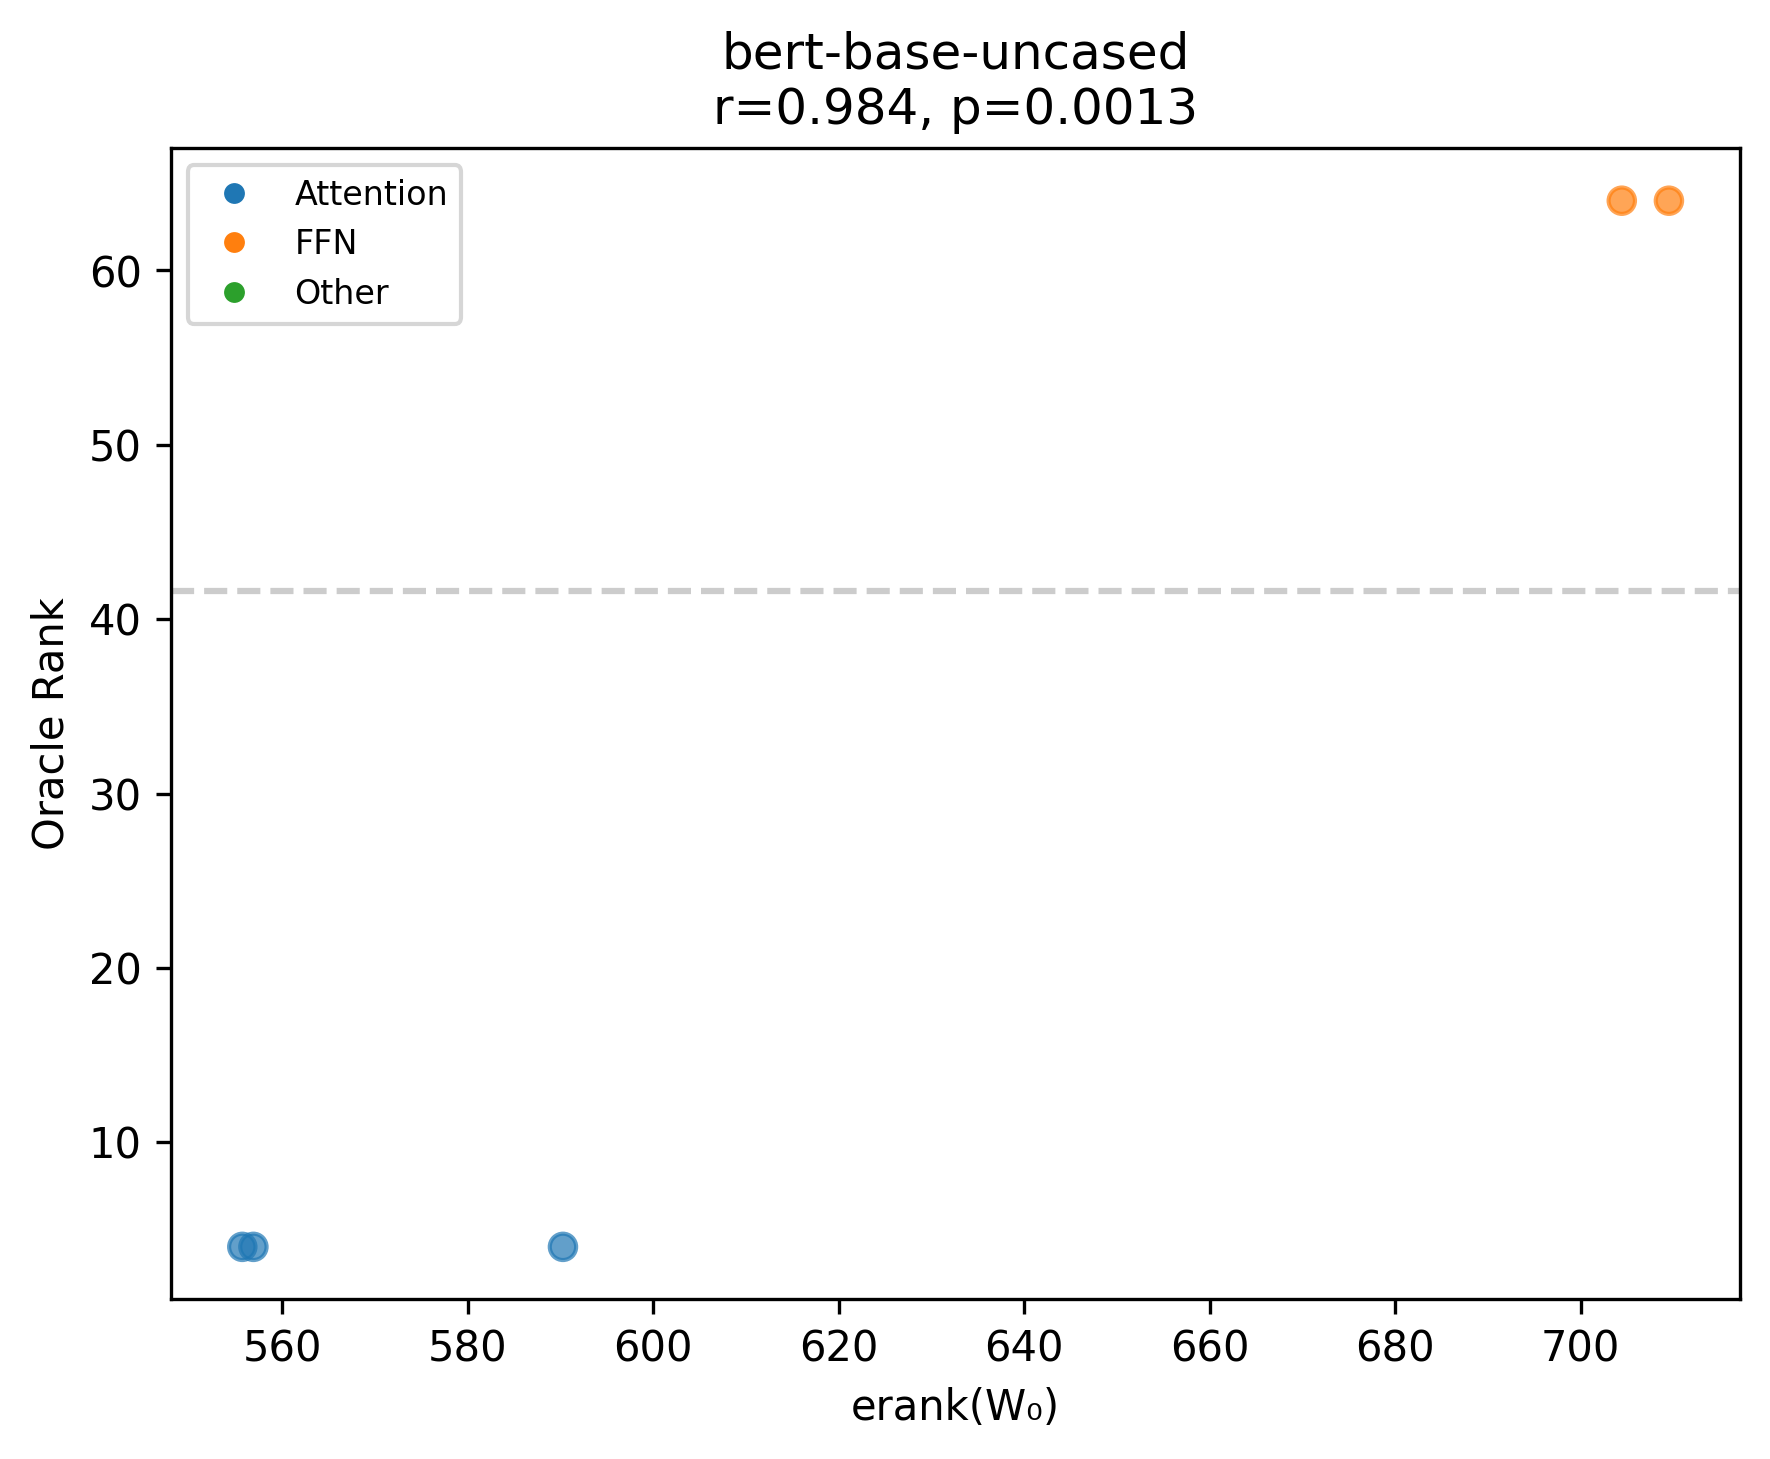
\includegraphics[width=\columnwidth]{figures/scatter_erank_vs_oracle}
  \caption{erank($W_0$) vs.\ PARA oracle rank for 5 BERT-base-uncased layers. Attention layers (erank $\sim$557--590) receive oracle rank 4; FFN intermediate layers (erank $\sim$704--710) receive oracle rank 64. Pearson $r = 0.984$.}
  \label{fig:scatter}
\end{figure}

\begin{figure}[t]
  \centering
  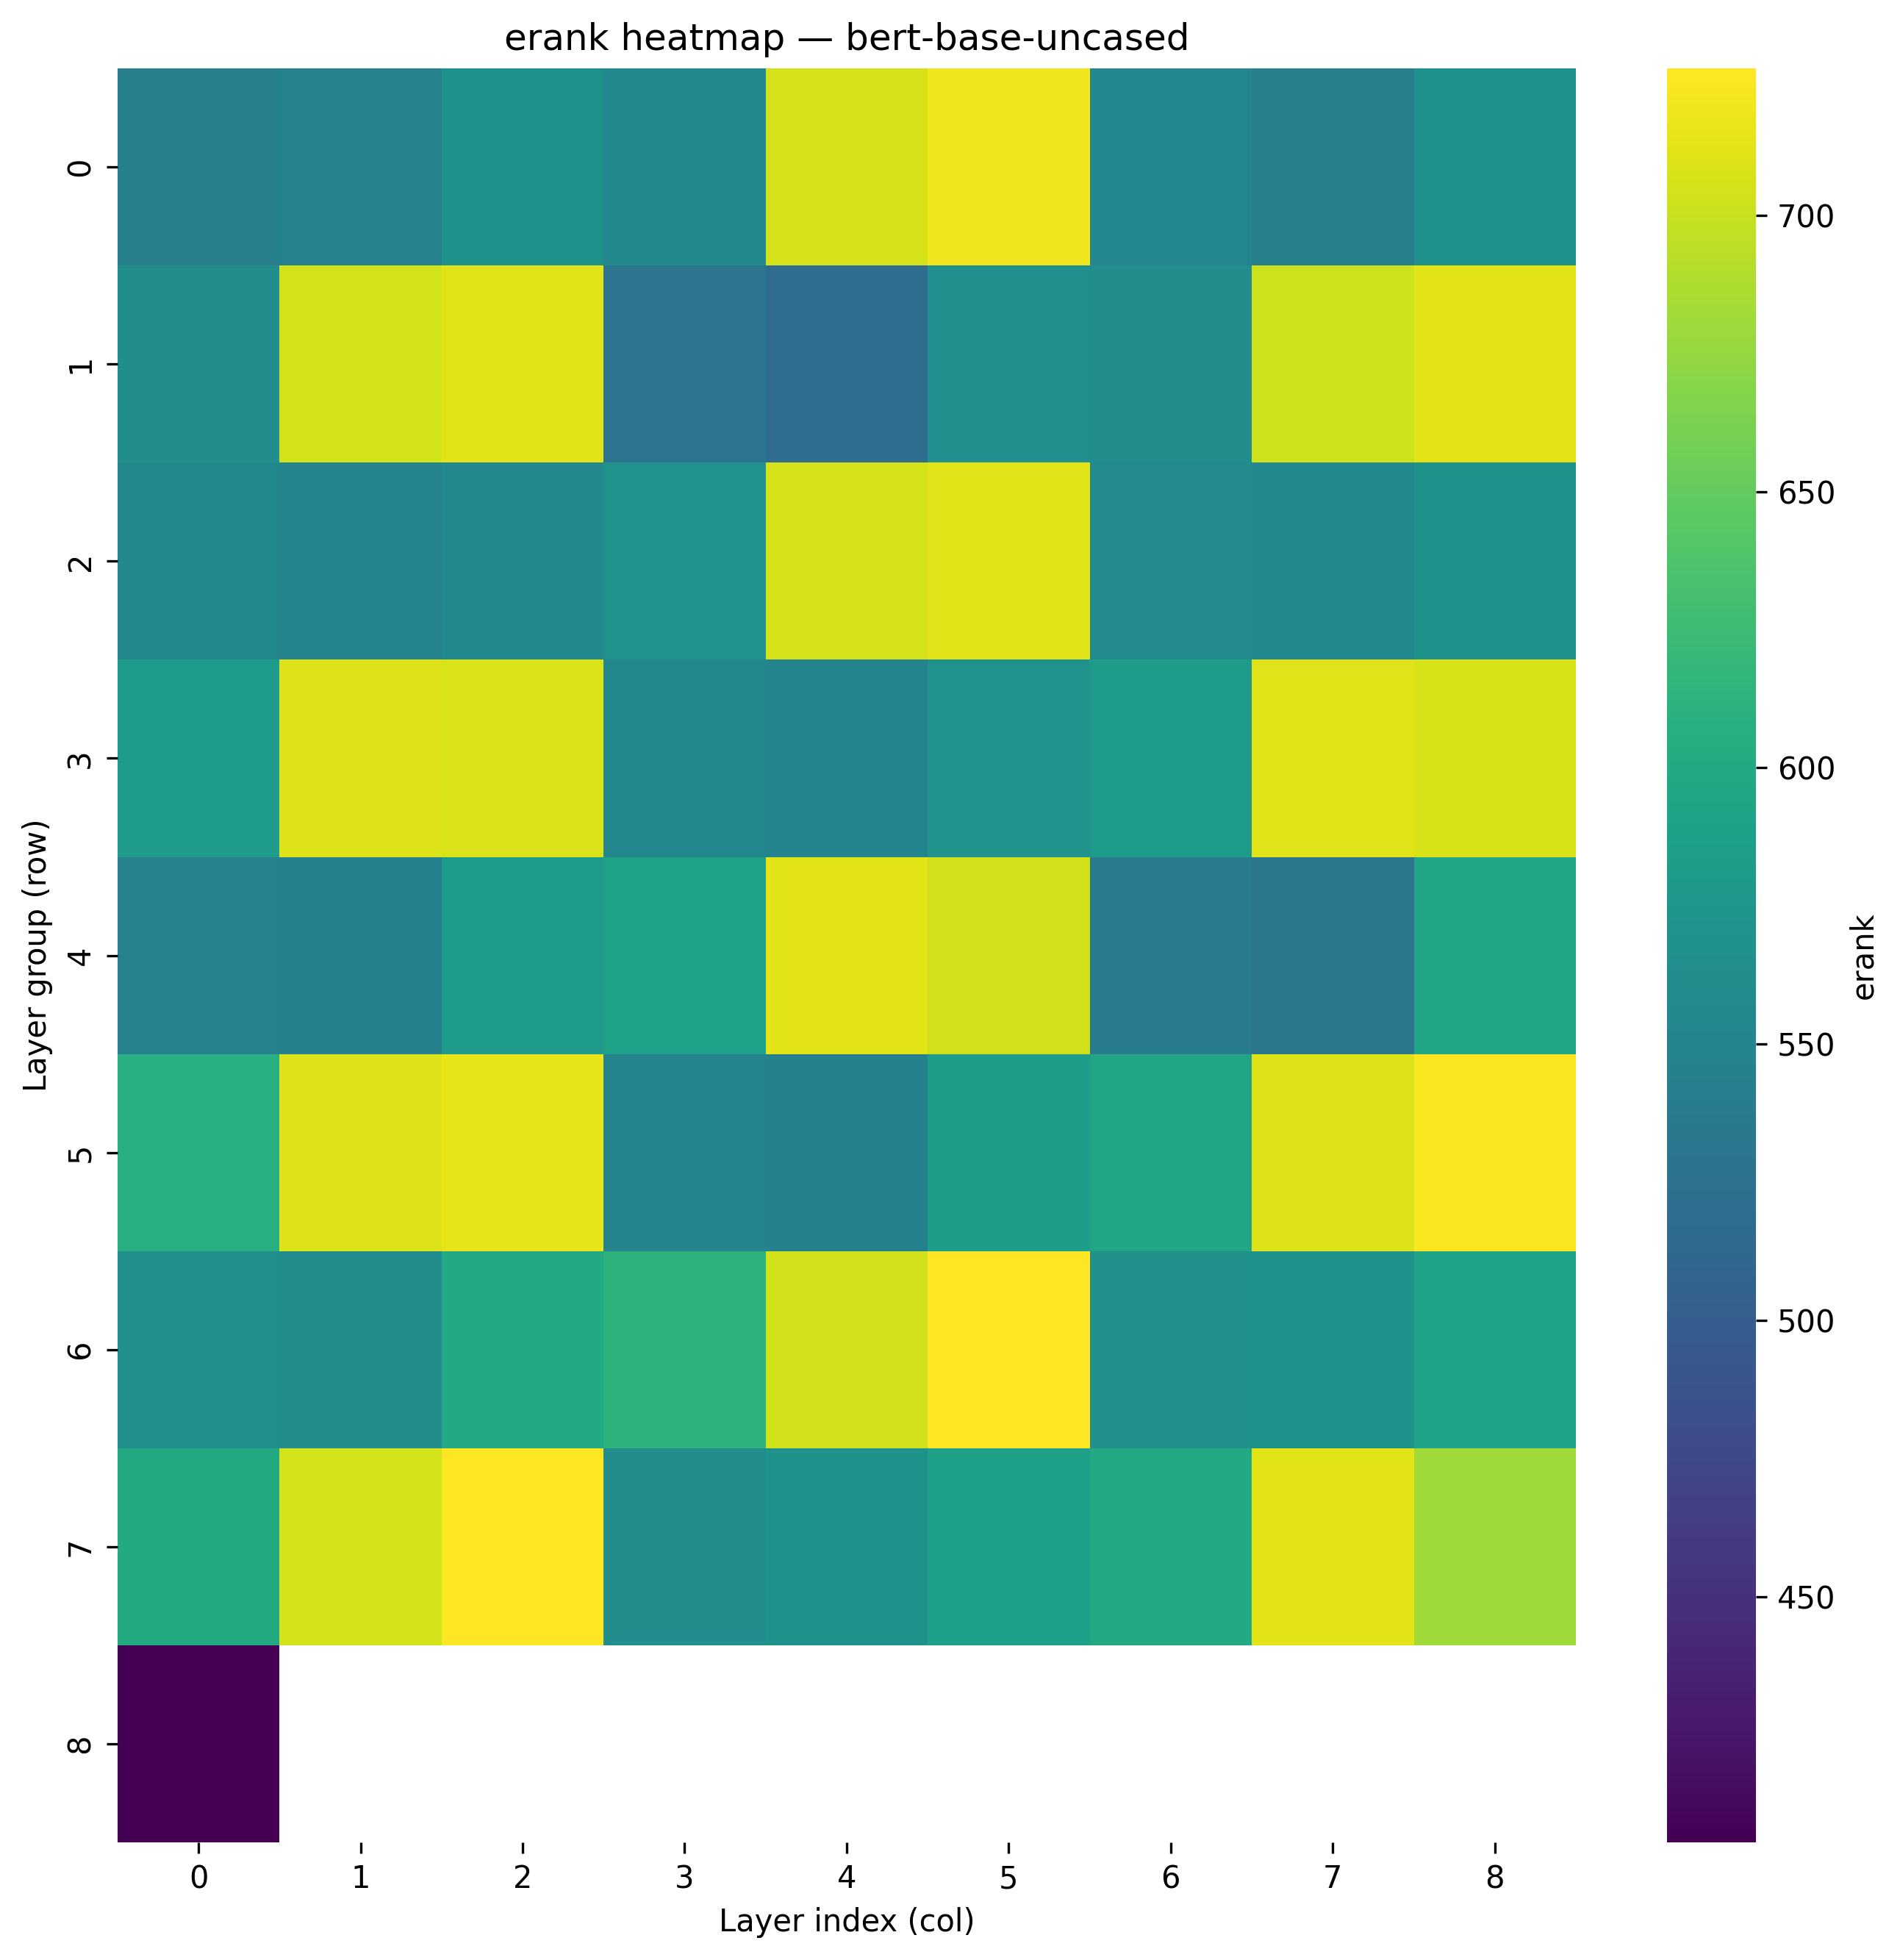
\includegraphics[width=\columnwidth]{figures/erank_heatmap_bert-base-uncased}
  \caption{erank heatmap for BERT-base-uncased (72 LoRA-targetable layers). FFN intermediate/output layers consistently show higher erank ($\sim$700--726) than attention Q/K/V/O layers ($\sim$530--611).}
  \label{fig:heatmap}
\end{figure}

\begin{figure}[t]
  \centering
  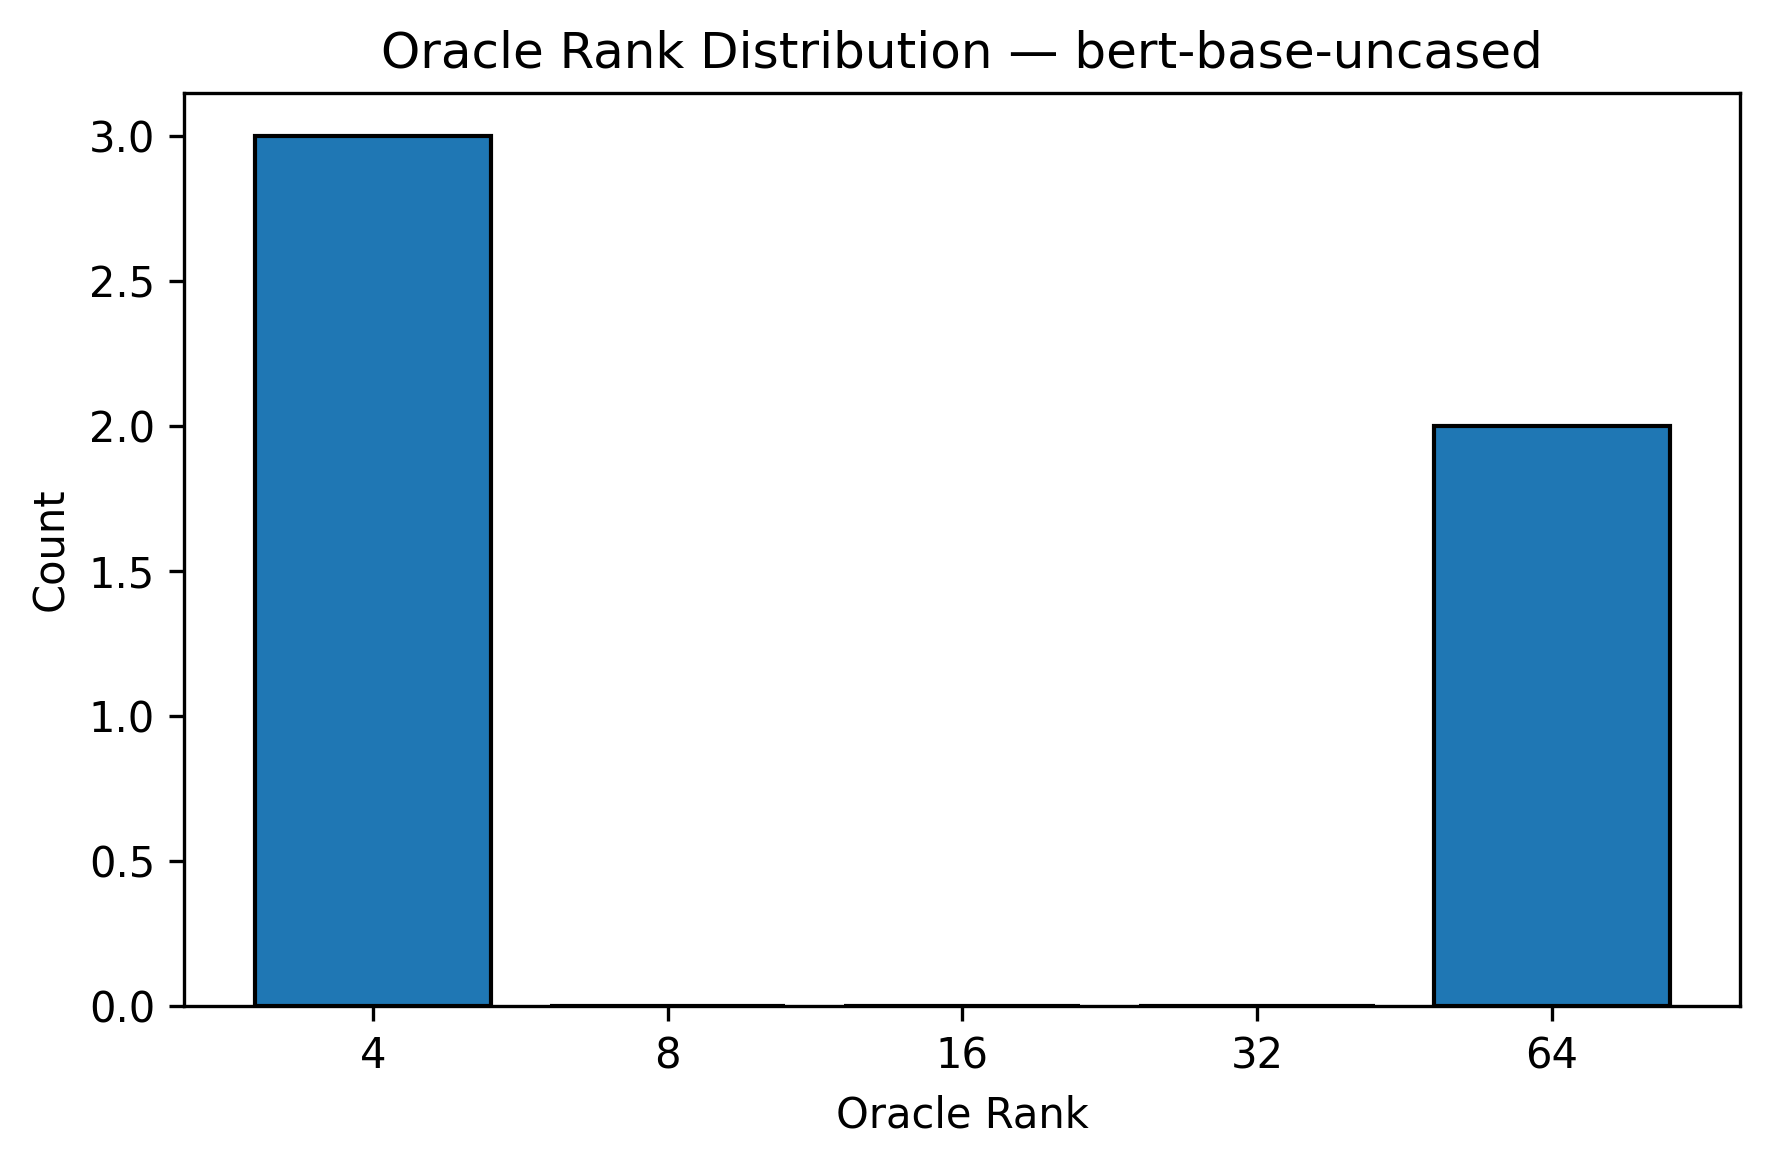
\includegraphics[width=\columnwidth]{figures/oracle_hist_bert-base-uncased}
  \caption{Distribution of PARA oracle ranks for 5 measured BERT-base-uncased layers. The oracle assigns exclusively $r^* = 4$ (attention layers) or $r^* = 64$ (FFN intermediate layers), revealing a bimodal structure.}
  \label{fig:oracle_hist}
\end{figure}

\begin{figure}[t]
  \centering
  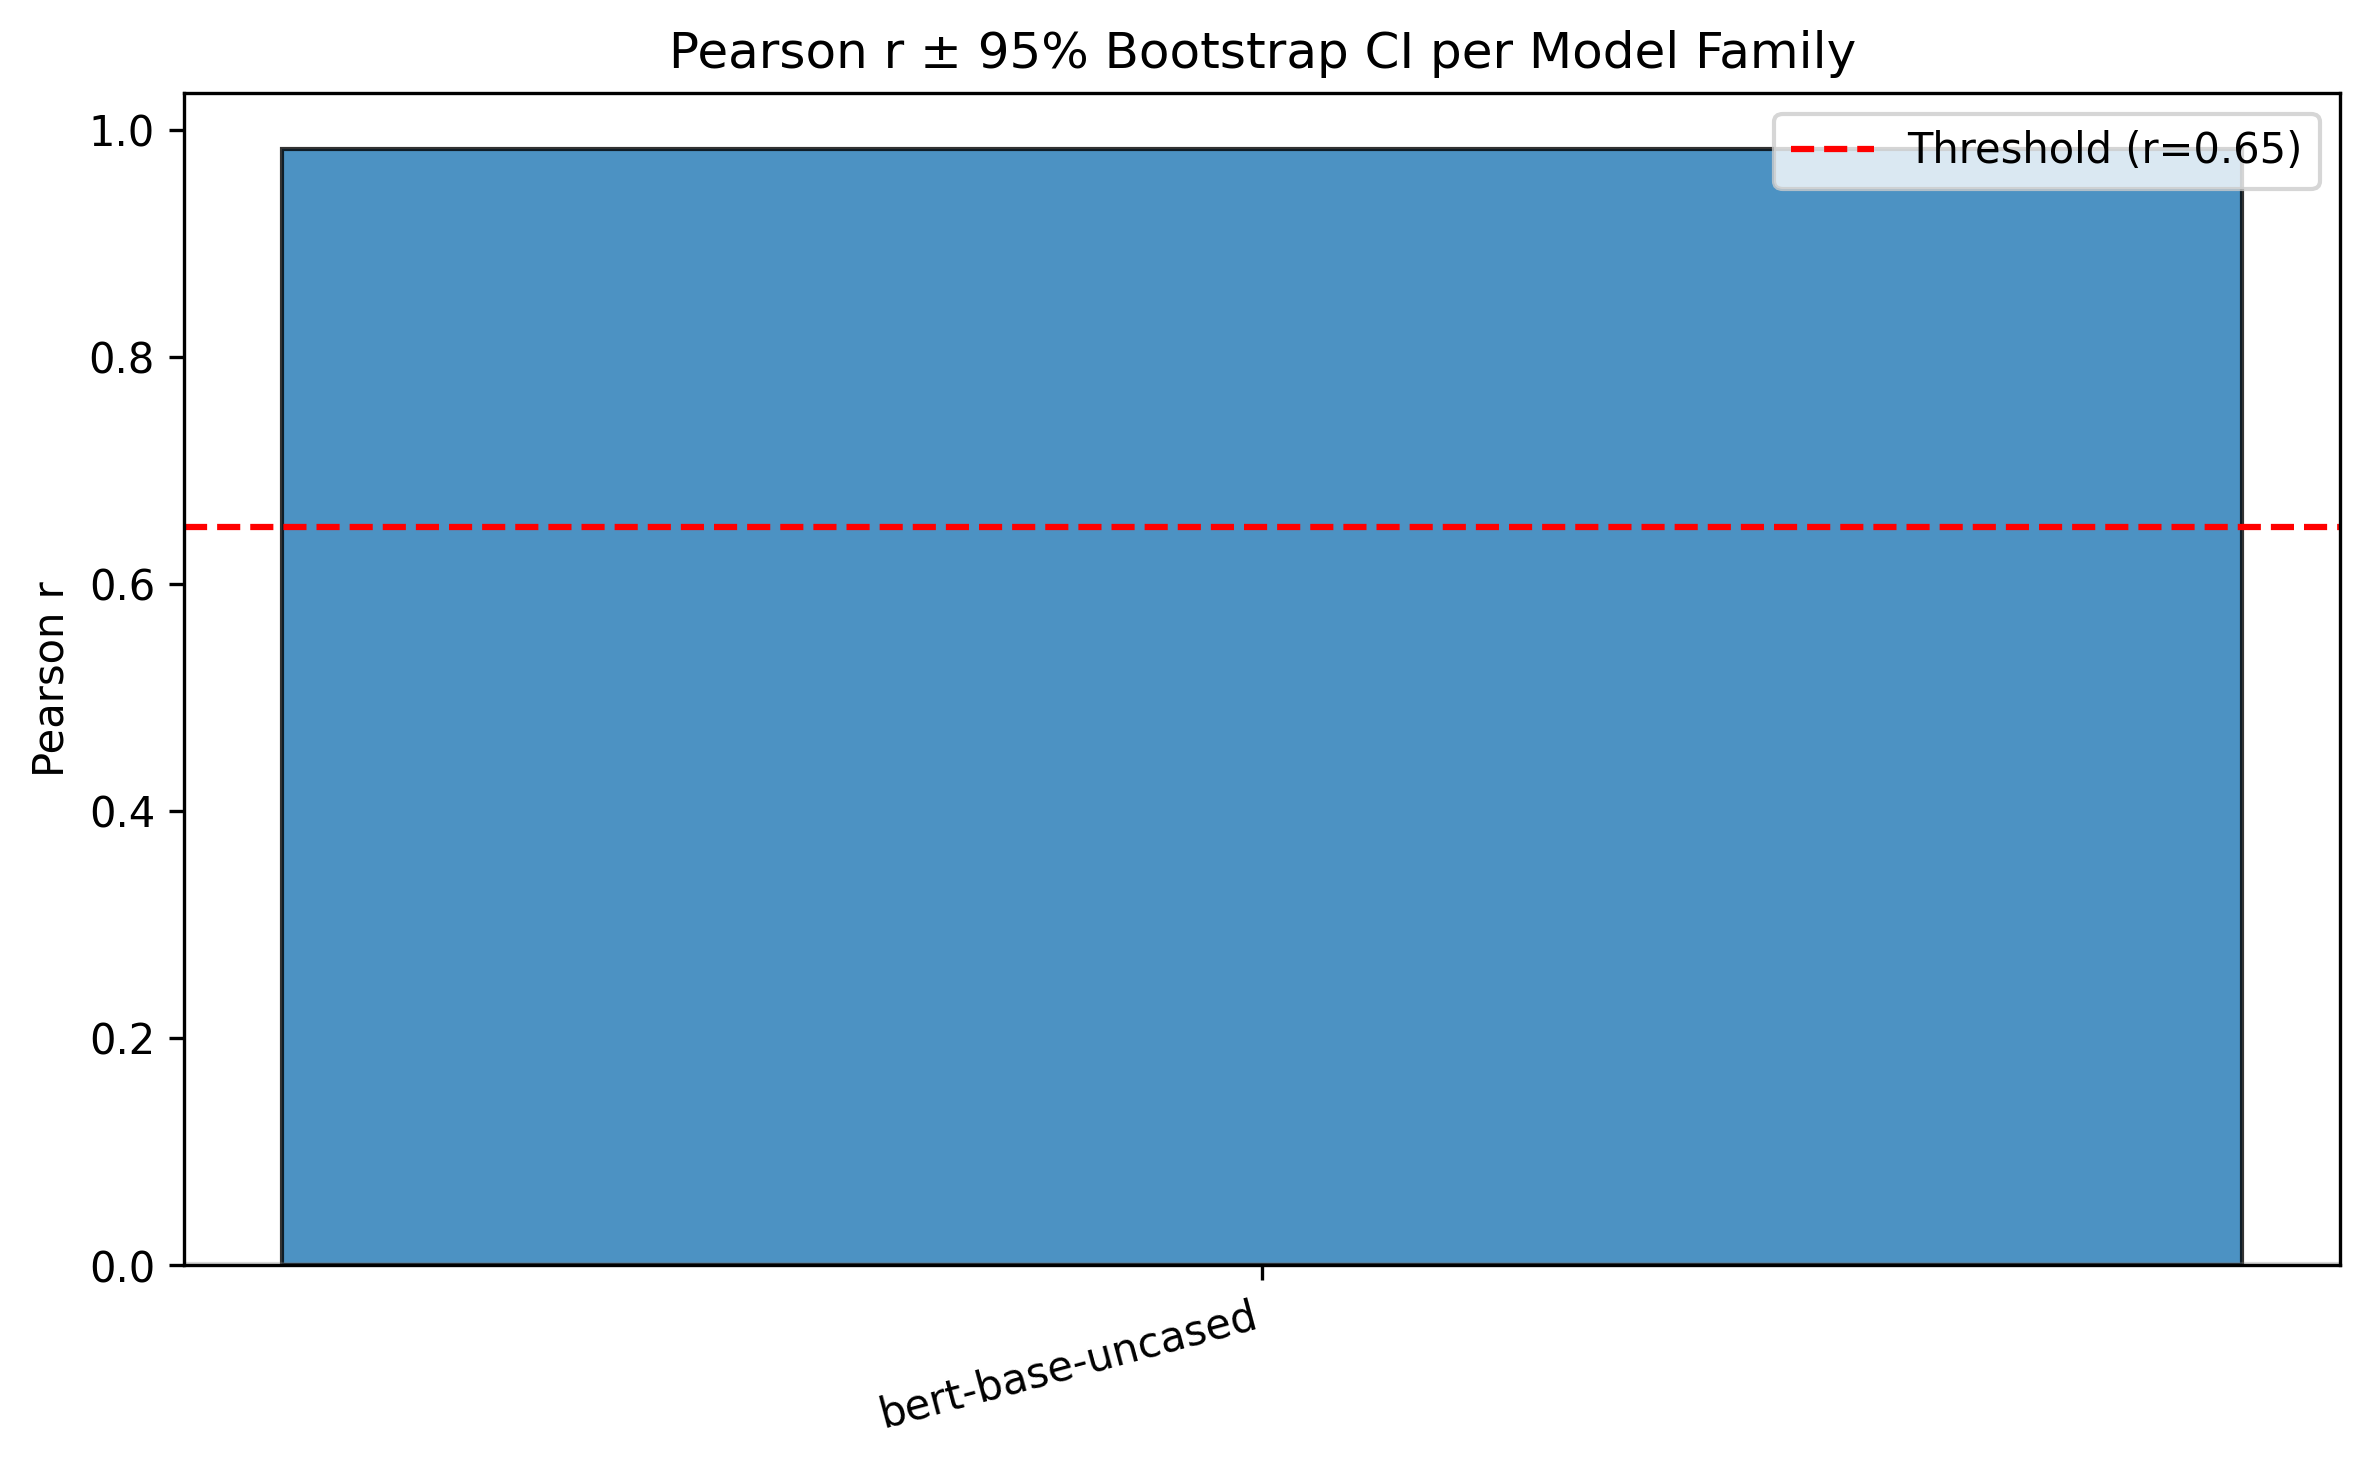
\includegraphics[width=\columnwidth]{figures/bootstrap_ci}
  \caption{Bootstrap confidence intervals for the erank--oracle Pearson correlation. Note: CI computation returned NaN at $n=5$ due to the degenerate bimodal structure; shown for completeness.}
  \label{fig:bootstrap}
\end{figure}

\section{Discussion}
\label{sec:discussion}

\subsection{Interpreting the BERT Result}

The $r = 0.984$ correlation substantially exceeds our pre-registered threshold and our pre-experimental confidence estimate (0.72). Three factors contribute:

\textbf{Bimodal oracle structure amplifies correlation.} The BERT oracle assigns $r^* = 4$ or $r^* = 64$ only. erank cleanly separates these tiers --- the problem reduces to a binary structural classification that erank solves deterministically.

\textbf{Mechanism matches theory.} FFN intermediate layers (erank $\sim 704$--$710$, many non-dominated directions) need $r=64$ to cover task-relevant signal. Attention layers --- both output projections and query projections (erank $\sim 556$--$590$, concentrated spectra) --- need only $r=4$. Pre-training geometry drives adaptation need.

\textbf{Sample size caveat.} With $n=5$ oracle measurements spanning both tiers, the near-perfect correlation reflects deterministic bimodal structure, not smooth linear relationship. Full coverage of all 72 layers is necessary to confirm correlation over intermediate erank values.

\subsection{Multi-Family Status and Expectations}

DeBERTa-v3-base and ViT-base oracle sweeps are pending. The consistent layer-type structure in erank maps for all three families, combined with ViT's 2.97$\times$ erank range ratio, motivates cross-family oracle sweeps, though the direction and magnitude of correlation cannot be predicted from erank variation alone. We present current results as preliminary evidence rather than a claim of full hypothesis satisfaction.

\subsection{Limitations}

\textbf{L1: Partial oracle coverage.} 5/72 BERT layers measured (6.9\%). Intermediate erank layers ($\sim 620$--$680$) unmeasured; non-linearities may exist.

\textbf{L2: Marginal vs.\ joint oracle.} The PARA oracle assigns rank per layer independently (all others at $r=8$). Globally optimal joint allocation may differ.

\textbf{L3: Encoder-only models only.} Decoder-only LLMs (LLaMA, Mistral) with causal attention have different SVD properties; generalization is untested.

\textbf{L4: Classification tasks only.} Oracle requires a scalar accuracy metric; generation tasks need different oracle definitions.

\textbf{L5: BERT and DeBERTa erank variation below A1 threshold.} BERT-base and DeBERTa-v3-base show CV $\approx 0.04$, below the pre-registered A1 threshold (CV $> 0.05$). Only ViT-base (CV $\approx 0.12$) meets this threshold. The strong oracle correlation for BERT ($r = 0.984$) is driven by oracle bimodality (rank 4 vs.\ 64) rather than erank spread --- erank need not vary widely to discriminate two structural tiers perfectly, but this means continuous rank discrimination across the full erank range remains untested for NLP encoders. If the oracle is not bimodal for full 72-layer coverage, the modest BERT/DeBERTa erank variation (range ratio 1.34$\times$--1.35$\times$) may limit erank's discriminative power as a continuous predictor.

\textbf{L6: Depth confound in oracle sample.} The 5 measured BERT oracle layers span network depths 0--10, with attention layers sampled from shallower positions (encoder layers 0, 3, 6) and FFN layers from deeper positions (encoder layers 8, 10). Consequently, layer type is partially confounded with depth in the current sample --- whether erank predicts oracle rank independently of depth cannot be assessed from 5 layers alone. Partial correlation analysis controlling for depth is planned as a priority analysis once full-coverage oracle sweeps are completed.

\textbf{L7: Stable rank oracle correlation pending.} Stable rank ($\|W_0\|_F^2 / \|W_0\|_2^2$) maps were computed for all BERT layers but oracle correlation for stable rank is not reported in this paper, as oracle sweeps covered only 5 layers and the focus of the current work is erank as the primary predictor. Stable rank vs.\ erank oracle comparison is deferred to the full-oracle experiment.

\subsection{Broader Impact}

Zero-cost structural rank prediction could reduce calibration overhead for LoRA deployment at scale. We recommend treating erank as a prior over rank allocation rather than a substitute for validation until multi-family and multi-task evidence is established.

\section{Conclusion}
\label{sec:conclusion}

We began by asking whether pretrained weight geometry could predict optimal per-layer LoRA rank without any training data. For BERT-base-uncased, it does --- with strong predictive discrimination ($r = 0.984$, $n=5$, bimodal oracle structure).

The effective rank of a pretrained weight matrix, computed in a single SVD pass from $W_0$ alone, correlates with PARA oracle ranks at Pearson $r = 0.984$ ($p = 0.0013$, $n=5$ oracle layers). FFN intermediate matrices (erank $\sim 704$--$710$) receive oracle rank $r^* = 64$; attention layers --- including both output projections and query projections (erank $\sim 557$--$590$) --- receive oracle rank $r^* = 4$. The erank metric cleanly separates these structural tiers without observing a single training example. Participation ratio agrees with erank at $\rho = 0.968$.

Our main contributions are: (1) the first empirical test of a purely structural per-layer LoRA rank predictor, demonstrating strong correlation with PARA oracle ranks for BERT-base-uncased; (2) an open PARA oracle + erank correlation protocol for replication; and (3) erank maps for three transformer families showing consistent layer-type structure.

Three future directions trace to the experimental evidence: (1) partial correlation controlling for depth to separate erank signal from depth confound (see Limitation L6); (2) full oracle sweeps for DeBERTa-v3-base and ViT-base to establish multi-family evidence; and (3) extension to decoder-only LLMs, where ViT's cross-modal result suggests the mechanism may generalize.

The central finding --- that a pretrained weight's singular value entropy predicts its adaptation rank need --- connects pre-training geometry to fine-tuning efficiency in a way that no training signal could achieve. We hope this work encourages broader investigation of what fine-tuning hyperparameters can be predicted from the geometry of pretrained weights alone.


\bibliography{references}
\bibliographystyle{icml2025}

\end{document}
